\documentclass[tikz,border=2pt]{standalone}
\usepackage{amsmath,amssymb}
\usetikzlibrary{positioning,arrows.meta,patterns}
\begin{document}
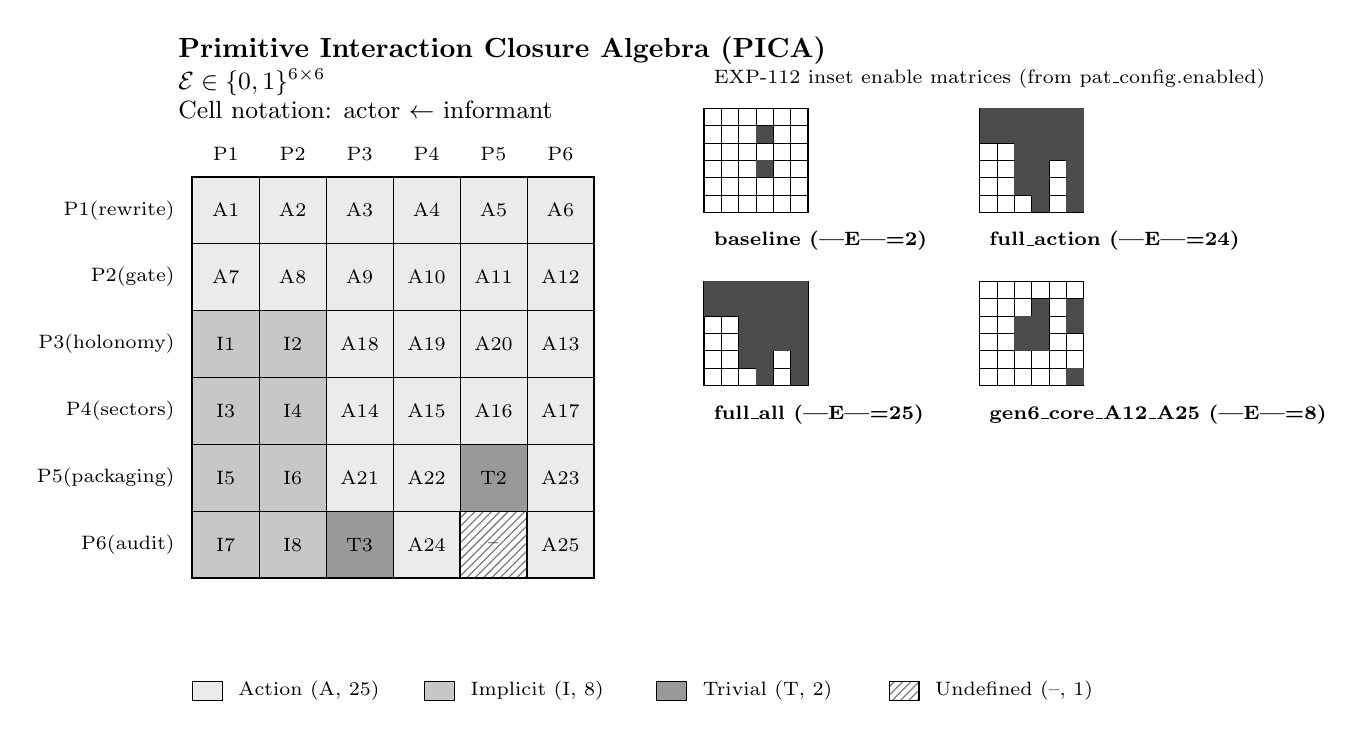
\begin{tikzpicture}[font=\small]
\def\cs{0.85}
\coordinate (G0) at (0,0);
\node[anchor=west,font=\bfseries] at (-0.3,6.70) {Primitive Interaction Closure Algebra (PICA)};
\node[anchor=west] at (-0.3,6.30) {$\mathcal{E}\in\{0,1\}^{6\times6}$};
\node[anchor=west] at (-0.3,5.95) {Cell notation: actor $\leftarrow$ informant};
\node[anchor=south,font=\scriptsize] at (0.5*\cs,5.18) {P1};
\node[anchor=south,font=\scriptsize] at (1.5*\cs,5.18) {P2};
\node[anchor=south,font=\scriptsize] at (2.5*\cs,5.18) {P3};
\node[anchor=south,font=\scriptsize] at (3.5*\cs,5.18) {P4};
\node[anchor=south,font=\scriptsize] at (4.5*\cs,5.18) {P5};
\node[anchor=south,font=\scriptsize] at (5.5*\cs,5.18) {P6};
\node[anchor=east,font=\scriptsize] at (-0.1,5.5*\cs) {P1(rewrite)};
\node[anchor=east,font=\scriptsize] at (-0.1,4.5*\cs) {P2(gate)};
\node[anchor=east,font=\scriptsize] at (-0.1,3.5*\cs) {P3(holonomy)};
\node[anchor=east,font=\scriptsize] at (-0.1,2.5*\cs) {P4(sectors)};
\node[anchor=east,font=\scriptsize] at (-0.1,1.5*\cs) {P5(packaging)};
\node[anchor=east,font=\scriptsize] at (-0.1,0.5*\cs) {P6(audit)};
\fill[black!8] (0*\cs,5*\cs) rectangle ++(\cs,\cs);
\draw[black,line width=0.3pt] (0*\cs,5*\cs) rectangle ++(\cs,\cs);
\node[font=\scriptsize] at (0.5*\cs,5.5*\cs) {A1};
\fill[black!8] (1*\cs,5*\cs) rectangle ++(\cs,\cs);
\draw[black,line width=0.3pt] (1*\cs,5*\cs) rectangle ++(\cs,\cs);
\node[font=\scriptsize] at (1.5*\cs,5.5*\cs) {A2};
\fill[black!8] (2*\cs,5*\cs) rectangle ++(\cs,\cs);
\draw[black,line width=0.3pt] (2*\cs,5*\cs) rectangle ++(\cs,\cs);
\node[font=\scriptsize] at (2.5*\cs,5.5*\cs) {A3};
\fill[black!8] (3*\cs,5*\cs) rectangle ++(\cs,\cs);
\draw[black,line width=0.3pt] (3*\cs,5*\cs) rectangle ++(\cs,\cs);
\node[font=\scriptsize] at (3.5*\cs,5.5*\cs) {A4};
\fill[black!8] (4*\cs,5*\cs) rectangle ++(\cs,\cs);
\draw[black,line width=0.3pt] (4*\cs,5*\cs) rectangle ++(\cs,\cs);
\node[font=\scriptsize] at (4.5*\cs,5.5*\cs) {A5};
\fill[black!8] (5*\cs,5*\cs) rectangle ++(\cs,\cs);
\draw[black,line width=0.3pt] (5*\cs,5*\cs) rectangle ++(\cs,\cs);
\node[font=\scriptsize] at (5.5*\cs,5.5*\cs) {A6};
\fill[black!8] (0*\cs,4*\cs) rectangle ++(\cs,\cs);
\draw[black,line width=0.3pt] (0*\cs,4*\cs) rectangle ++(\cs,\cs);
\node[font=\scriptsize] at (0.5*\cs,4.5*\cs) {A7};
\fill[black!8] (1*\cs,4*\cs) rectangle ++(\cs,\cs);
\draw[black,line width=0.3pt] (1*\cs,4*\cs) rectangle ++(\cs,\cs);
\node[font=\scriptsize] at (1.5*\cs,4.5*\cs) {A8};
\fill[black!8] (2*\cs,4*\cs) rectangle ++(\cs,\cs);
\draw[black,line width=0.3pt] (2*\cs,4*\cs) rectangle ++(\cs,\cs);
\node[font=\scriptsize] at (2.5*\cs,4.5*\cs) {A9};
\fill[black!8] (3*\cs,4*\cs) rectangle ++(\cs,\cs);
\draw[black,line width=0.3pt] (3*\cs,4*\cs) rectangle ++(\cs,\cs);
\node[font=\scriptsize] at (3.5*\cs,4.5*\cs) {A10};
\fill[black!8] (4*\cs,4*\cs) rectangle ++(\cs,\cs);
\draw[black,line width=0.3pt] (4*\cs,4*\cs) rectangle ++(\cs,\cs);
\node[font=\scriptsize] at (4.5*\cs,4.5*\cs) {A11};
\fill[black!8] (5*\cs,4*\cs) rectangle ++(\cs,\cs);
\draw[black,line width=0.3pt] (5*\cs,4*\cs) rectangle ++(\cs,\cs);
\node[font=\scriptsize] at (5.5*\cs,4.5*\cs) {A12};
\fill[black!22] (0*\cs,3*\cs) rectangle ++(\cs,\cs);
\draw[black,line width=0.3pt] (0*\cs,3*\cs) rectangle ++(\cs,\cs);
\node[font=\scriptsize] at (0.5*\cs,3.5*\cs) {I1};
\fill[black!22] (1*\cs,3*\cs) rectangle ++(\cs,\cs);
\draw[black,line width=0.3pt] (1*\cs,3*\cs) rectangle ++(\cs,\cs);
\node[font=\scriptsize] at (1.5*\cs,3.5*\cs) {I2};
\fill[black!8] (2*\cs,3*\cs) rectangle ++(\cs,\cs);
\draw[black,line width=0.3pt] (2*\cs,3*\cs) rectangle ++(\cs,\cs);
\node[font=\scriptsize] at (2.5*\cs,3.5*\cs) {A18};
\fill[black!8] (3*\cs,3*\cs) rectangle ++(\cs,\cs);
\draw[black,line width=0.3pt] (3*\cs,3*\cs) rectangle ++(\cs,\cs);
\node[font=\scriptsize] at (3.5*\cs,3.5*\cs) {A19};
\fill[black!8] (4*\cs,3*\cs) rectangle ++(\cs,\cs);
\draw[black,line width=0.3pt] (4*\cs,3*\cs) rectangle ++(\cs,\cs);
\node[font=\scriptsize] at (4.5*\cs,3.5*\cs) {A20};
\fill[black!8] (5*\cs,3*\cs) rectangle ++(\cs,\cs);
\draw[black,line width=0.3pt] (5*\cs,3*\cs) rectangle ++(\cs,\cs);
\node[font=\scriptsize] at (5.5*\cs,3.5*\cs) {A13};
\fill[black!22] (0*\cs,2*\cs) rectangle ++(\cs,\cs);
\draw[black,line width=0.3pt] (0*\cs,2*\cs) rectangle ++(\cs,\cs);
\node[font=\scriptsize] at (0.5*\cs,2.5*\cs) {I3};
\fill[black!22] (1*\cs,2*\cs) rectangle ++(\cs,\cs);
\draw[black,line width=0.3pt] (1*\cs,2*\cs) rectangle ++(\cs,\cs);
\node[font=\scriptsize] at (1.5*\cs,2.5*\cs) {I4};
\fill[black!8] (2*\cs,2*\cs) rectangle ++(\cs,\cs);
\draw[black,line width=0.3pt] (2*\cs,2*\cs) rectangle ++(\cs,\cs);
\node[font=\scriptsize] at (2.5*\cs,2.5*\cs) {A14};
\fill[black!8] (3*\cs,2*\cs) rectangle ++(\cs,\cs);
\draw[black,line width=0.3pt] (3*\cs,2*\cs) rectangle ++(\cs,\cs);
\node[font=\scriptsize] at (3.5*\cs,2.5*\cs) {A15};
\fill[black!8] (4*\cs,2*\cs) rectangle ++(\cs,\cs);
\draw[black,line width=0.3pt] (4*\cs,2*\cs) rectangle ++(\cs,\cs);
\node[font=\scriptsize] at (4.5*\cs,2.5*\cs) {A16};
\fill[black!8] (5*\cs,2*\cs) rectangle ++(\cs,\cs);
\draw[black,line width=0.3pt] (5*\cs,2*\cs) rectangle ++(\cs,\cs);
\node[font=\scriptsize] at (5.5*\cs,2.5*\cs) {A17};
\fill[black!22] (0*\cs,1*\cs) rectangle ++(\cs,\cs);
\draw[black,line width=0.3pt] (0*\cs,1*\cs) rectangle ++(\cs,\cs);
\node[font=\scriptsize] at (0.5*\cs,1.5*\cs) {I5};
\fill[black!22] (1*\cs,1*\cs) rectangle ++(\cs,\cs);
\draw[black,line width=0.3pt] (1*\cs,1*\cs) rectangle ++(\cs,\cs);
\node[font=\scriptsize] at (1.5*\cs,1.5*\cs) {I6};
\fill[black!8] (2*\cs,1*\cs) rectangle ++(\cs,\cs);
\draw[black,line width=0.3pt] (2*\cs,1*\cs) rectangle ++(\cs,\cs);
\node[font=\scriptsize] at (2.5*\cs,1.5*\cs) {A21};
\fill[black!8] (3*\cs,1*\cs) rectangle ++(\cs,\cs);
\draw[black,line width=0.3pt] (3*\cs,1*\cs) rectangle ++(\cs,\cs);
\node[font=\scriptsize] at (3.5*\cs,1.5*\cs) {A22};
\fill[black!40] (4*\cs,1*\cs) rectangle ++(\cs,\cs);
\draw[black,line width=0.3pt] (4*\cs,1*\cs) rectangle ++(\cs,\cs);
\node[font=\scriptsize] at (4.5*\cs,1.5*\cs) {T2};
\fill[black!8] (5*\cs,1*\cs) rectangle ++(\cs,\cs);
\draw[black,line width=0.3pt] (5*\cs,1*\cs) rectangle ++(\cs,\cs);
\node[font=\scriptsize] at (5.5*\cs,1.5*\cs) {A23};
\fill[black!22] (0*\cs,0*\cs) rectangle ++(\cs,\cs);
\draw[black,line width=0.3pt] (0*\cs,0*\cs) rectangle ++(\cs,\cs);
\node[font=\scriptsize] at (0.5*\cs,0.5*\cs) {I7};
\fill[black!22] (1*\cs,0*\cs) rectangle ++(\cs,\cs);
\draw[black,line width=0.3pt] (1*\cs,0*\cs) rectangle ++(\cs,\cs);
\node[font=\scriptsize] at (1.5*\cs,0.5*\cs) {I8};
\fill[black!40] (2*\cs,0*\cs) rectangle ++(\cs,\cs);
\draw[black,line width=0.3pt] (2*\cs,0*\cs) rectangle ++(\cs,\cs);
\node[font=\scriptsize] at (2.5*\cs,0.5*\cs) {T3};
\fill[black!8] (3*\cs,0*\cs) rectangle ++(\cs,\cs);
\draw[black,line width=0.3pt] (3*\cs,0*\cs) rectangle ++(\cs,\cs);
\node[font=\scriptsize] at (3.5*\cs,0.5*\cs) {A24};
\fill[white] (4*\cs,0*\cs) rectangle ++(\cs,\cs);
\draw[pattern=north east lines,pattern color=black!55] (4*\cs,0*\cs) rectangle ++(\cs,\cs);
\draw[black,line width=0.3pt] (4*\cs,0*\cs) rectangle ++(\cs,\cs);
\node[font=\scriptsize] at (4.5*\cs,0.5*\cs) {--};
\fill[black!8] (5*\cs,0*\cs) rectangle ++(\cs,\cs);
\draw[black,line width=0.3pt] (5*\cs,0*\cs) rectangle ++(\cs,\cs);
\node[font=\scriptsize] at (5.5*\cs,0.5*\cs) {A25};
\draw[line width=0.7pt] (0,0) rectangle (6*\cs,6*\cs);
\begin{scope}[shift={(0,-1.55)}]
\fill[black!8] (0.0,0) rectangle ++(0.38,0.24);
\draw (0.0,0) rectangle ++(0.38,0.24);
\node[anchor=west,font=\scriptsize] at (0.46,0.12) {Action (A, 25)};
\fill[black!22] (2.95,0) rectangle ++(0.38,0.24);
\draw (2.95,0) rectangle ++(0.38,0.24);
\node[anchor=west,font=\scriptsize] at (3.41,0.12) {Implicit (I, 8)};
\fill[black!40] (5.9,0) rectangle ++(0.38,0.24);
\draw (5.9,0) rectangle ++(0.38,0.24);
\node[anchor=west,font=\scriptsize] at (6.36,0.12) {Trivial (T, 2)};
\fill[white] (8.850000000000001,0) rectangle ++(0.38,0.24);
\draw[pattern=north east lines,pattern color=black!55] (8.850000000000001,0) rectangle ++(0.38,0.24);
\draw (8.850000000000001,0) rectangle ++(0.38,0.24);
\node[anchor=west,font=\scriptsize] at (9.310000000000002,0.12) {Undefined (--, 1)};
\end{scope}
\newcommand{\InsetGrid}[3]{% #1 x, #2 y, #3 title
  \begin{scope}[shift={(#1,#2)}]
  \def\is{0.22}
  \node[anchor=north west,font=\scriptsize\bfseries] at (0,-0.12) {#3};
  \draw[line width=0.45pt] (0,0) rectangle (6*\is,6*\is);
  \foreach \i in {1,...,5} {\draw[line width=0.2pt] (\i*\is,0) -- (\i*\is,6*\is);}
  \foreach \j in {1,...,5} {\draw[line width=0.2pt] (0,\j*\is) -- (6*\is,\j*\is);}
  \end{scope}%
}
\InsetGrid{6.5}{4.65}{baseline (|E|=2)}
\fill[black!70] (7.160,5.530) rectangle ++(0.22,0.22);
\fill[black!70] (7.160,5.090) rectangle ++(0.22,0.22);
\begin{scope}[shift={(0.8,0)}] % shift right column for title clearance
\InsetGrid{9.2}{4.65}{full\_action (|E|=24)}
\fill[black!70] (9.200,5.750) rectangle ++(0.22,0.22);
\fill[black!70] (9.420,5.750) rectangle ++(0.22,0.22);
\fill[black!70] (9.640,5.750) rectangle ++(0.22,0.22);
\fill[black!70] (9.860,5.750) rectangle ++(0.22,0.22);
\fill[black!70] (10.080,5.750) rectangle ++(0.22,0.22);
\fill[black!70] (10.300,5.750) rectangle ++(0.22,0.22);
\fill[black!70] (9.200,5.530) rectangle ++(0.22,0.22);
\fill[black!70] (9.420,5.530) rectangle ++(0.22,0.22);
\fill[black!70] (9.640,5.530) rectangle ++(0.22,0.22);
\fill[black!70] (9.860,5.530) rectangle ++(0.22,0.22);
\fill[black!70] (10.080,5.530) rectangle ++(0.22,0.22);
\fill[black!70] (10.300,5.530) rectangle ++(0.22,0.22);
\fill[black!70] (9.640,5.310) rectangle ++(0.22,0.22);
\fill[black!70] (9.860,5.310) rectangle ++(0.22,0.22);
\fill[black!70] (10.080,5.310) rectangle ++(0.22,0.22);
\fill[black!70] (10.300,5.310) rectangle ++(0.22,0.22);
\fill[black!70] (9.640,5.090) rectangle ++(0.22,0.22);
\fill[black!70] (9.860,5.090) rectangle ++(0.22,0.22);
\fill[black!70] (10.300,5.090) rectangle ++(0.22,0.22);
\fill[black!70] (9.640,4.870) rectangle ++(0.22,0.22);
\fill[black!70] (9.860,4.870) rectangle ++(0.22,0.22);
\fill[black!70] (10.300,4.870) rectangle ++(0.22,0.22);
\fill[black!70] (9.860,4.650) rectangle ++(0.22,0.22);
\fill[black!70] (10.300,4.650) rectangle ++(0.22,0.22);
\end{scope}
\InsetGrid{6.5}{2.45}{full\_all (|E|=25)}
\fill[black!70] (6.500,3.550) rectangle ++(0.22,0.22);
\fill[black!70] (6.720,3.550) rectangle ++(0.22,0.22);
\fill[black!70] (6.940,3.550) rectangle ++(0.22,0.22);
\fill[black!70] (7.160,3.550) rectangle ++(0.22,0.22);
\fill[black!70] (7.380,3.550) rectangle ++(0.22,0.22);
\fill[black!70] (7.600,3.550) rectangle ++(0.22,0.22);
\fill[black!70] (6.500,3.330) rectangle ++(0.22,0.22);
\fill[black!70] (6.720,3.330) rectangle ++(0.22,0.22);
\fill[black!70] (6.940,3.330) rectangle ++(0.22,0.22);
\fill[black!70] (7.160,3.330) rectangle ++(0.22,0.22);
\fill[black!70] (7.380,3.330) rectangle ++(0.22,0.22);
\fill[black!70] (7.600,3.330) rectangle ++(0.22,0.22);
\fill[black!70] (6.940,3.110) rectangle ++(0.22,0.22);
\fill[black!70] (7.160,3.110) rectangle ++(0.22,0.22);
\fill[black!70] (7.380,3.110) rectangle ++(0.22,0.22);
\fill[black!70] (7.600,3.110) rectangle ++(0.22,0.22);
\fill[black!70] (6.940,2.890) rectangle ++(0.22,0.22);
\fill[black!70] (7.160,2.890) rectangle ++(0.22,0.22);
\fill[black!70] (7.380,2.890) rectangle ++(0.22,0.22);
\fill[black!70] (7.600,2.890) rectangle ++(0.22,0.22);
\fill[black!70] (6.940,2.670) rectangle ++(0.22,0.22);
\fill[black!70] (7.160,2.670) rectangle ++(0.22,0.22);
\fill[black!70] (7.600,2.670) rectangle ++(0.22,0.22);
\fill[black!70] (7.160,2.450) rectangle ++(0.22,0.22);
\fill[black!70] (7.600,2.450) rectangle ++(0.22,0.22);
\begin{scope}[shift={(0.8,0)}] % shift right column for title clearance
\InsetGrid{9.2}{2.45}{gen6\_core\_A12\_A25 (|E|=8)}
\fill[black!70] (9.860,3.330) rectangle ++(0.22,0.22);
\fill[black!70] (10.300,3.330) rectangle ++(0.22,0.22);
\fill[black!70] (9.640,3.110) rectangle ++(0.22,0.22);
\fill[black!70] (9.860,3.110) rectangle ++(0.22,0.22);
\fill[black!70] (10.300,3.110) rectangle ++(0.22,0.22);
\fill[black!70] (9.640,2.890) rectangle ++(0.22,0.22);
\fill[black!70] (9.860,2.890) rectangle ++(0.22,0.22);
\fill[black!70] (10.300,2.450) rectangle ++(0.22,0.22);
\end{scope}
\node[anchor=west,font=\scriptsize] at (6.5,6.35) {EXP-112 inset enable matrices (from $\mathrm{pat\_config.enabled}$)};
\end{tikzpicture}
\end{document}
